This search \cite{CMS:2016nhb} looks for evidence of SUSY in events with jets identified as top quarks. An excess of events containing top-tagged jets (top tags) over the standard model background may be evidence of the production of top squark pairs, whose existence has been motivated as a solution to the hierarchy problem (Section \ref{sec:problems}).  The possibility of top squarks in mass range below about 450 GeV has largely been ruled out by results from other experiments.  However, considerations of naturalness implore us to look for evidence of top squarks nonetheless. The analysis is optimized to be sensitive to signatures resembling the simplified models shown in Fig. \ref{fig:hadstopSMS}.
\begin{figure}[h]
\centering
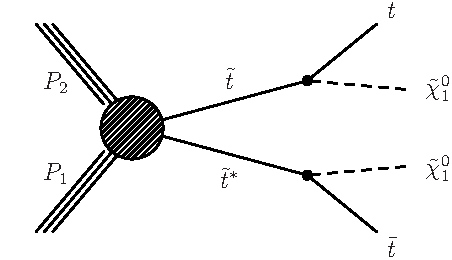
\includegraphics[width=0.45\textwidth]{figures/SusySearches/HadStop2015/T2tt.pdf}
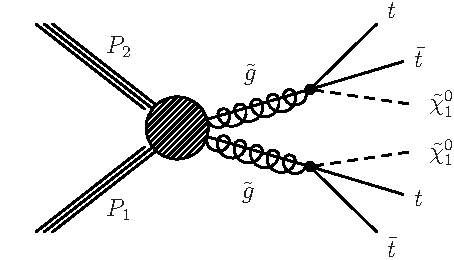
\includegraphics[width=0.45\textwidth]{figures/SusySearches/HadStop2015/T1tttt.pdf}\\
\caption{
  The simplified models used for the optimization and interpretation of the hadronic search for SUSY in events with top-tagged jets. They are T2tt (left) and T1tttt (right).
}
\label{fig:hadstopSMS}
\end{figure}

In addition to the multiplicity of top tags, other observables are used for signal/background discrimination, including the $\Ht$, $\met$, $\njets$, $\nbjets$, and the stransverse mass $M_{\text{T2}}$~\cite{Lester:1999tx}. Top tags are constructed by considering all three-jet combinations in an event, and selecting a combination with an invariant mass consistent with the top quark mass. Additional topological requirements are placed on the top-tagged jet to reject background from QCD jet combinations. After identifying a top-tagged jet, the remaining jets in the event are analyzed and checked for consistency with a second top quark in the event, inferred by the presence of a b-tagged jet. In the event that both systems (the top-tagged system and the remnant b-tagged jet) are reconstructed, the $M_{\text{T2}}$ is computed taking the four-vectors of the two systems as input, along with the $\met$ of the event. 

Events are collected using the same hadronic trigger used in the work of the previous section,
\begin{itemize}
  \item \texttt{HLT\_PFHT350\_PFMET100\_*}.
\end{itemize}
The probability for the trigger to accept an event that passes the baseline selection is greater than 98\%. For the baseline selection, events are selected if they have
\begin{itemize}
\item no reconstructed, isolated muon with a $\pt>10$ GeV, $|\eta|<2.4$, and isolation $<0.2$;
\item no reconstructed, isolated electron with a $\pt>10$ GeV, $|\eta|<2.5$, and isolation $<0.1$;
\item no reconstructed, isolated lepton (hadron) track with a $\pt>5$ (10) GeV, $|\eta|<2.5$, and isolation $0.2$;
\item $\Ht>500$ GeV;
\item $\met>200$ GeV;
\item $\Delta\phi(\mht$, jet$_{1,2,3})>$ 0.5, 0.5, 0.3;
\item $N_t\geq1$, where $N_t$ is multiplicity of top tags;
\item $\nbjets\geq1$, and
\item $M_{\text{T2}}>200$ GeV.
\end{itemize}
After the baseline selection, events are further subdivided into 37 search bins defined by rectangular boundaries in the dimensions of $\met$, $M_{\text{T2}}$, $\nbjets$, and $N_t$, with boundaries and bin numbers shown in Fig. \ref{fig:hadstopArray}.
\begin{figure}[h]
  \begin{center}
    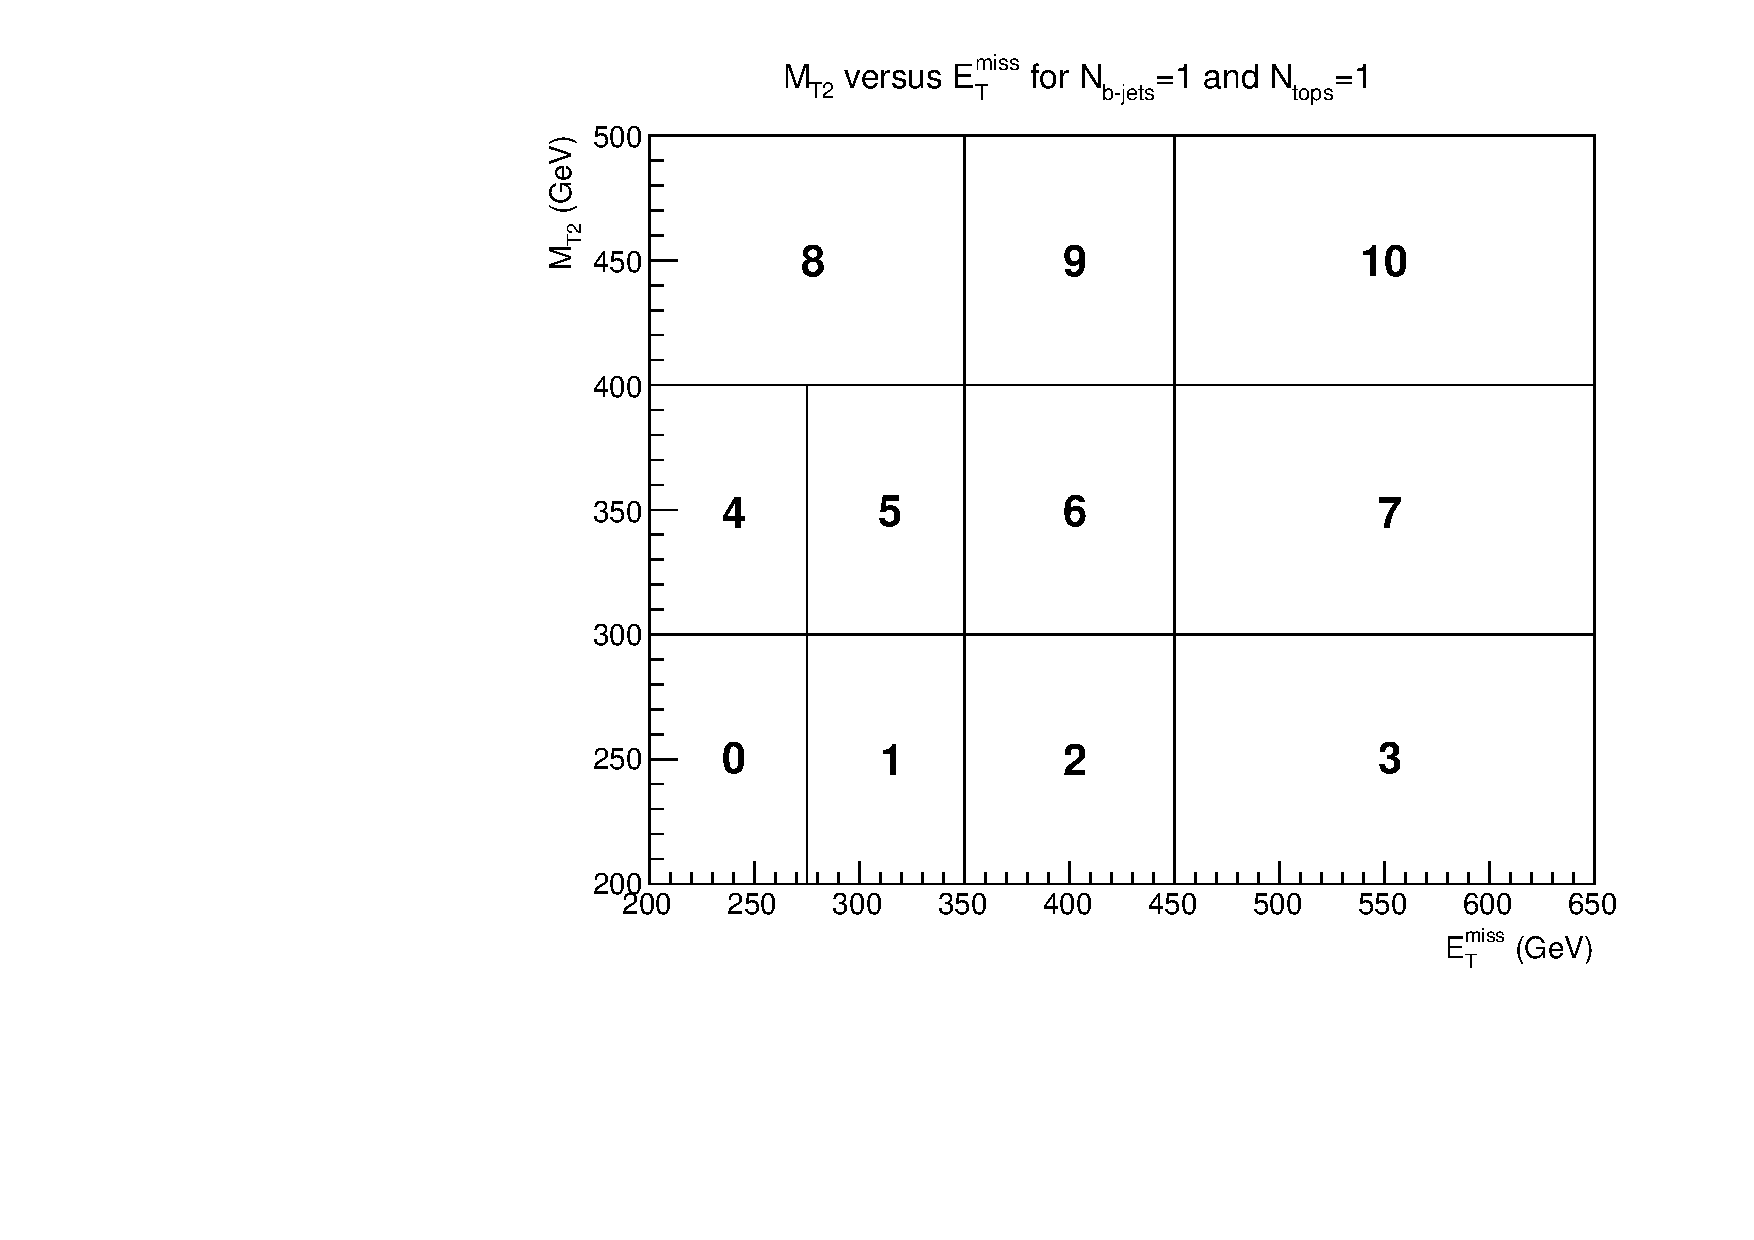
\includegraphics[width=0.45\linewidth]{HadStopPaper/figures/poly_MT2_vs_met_merged_0.pdf}
    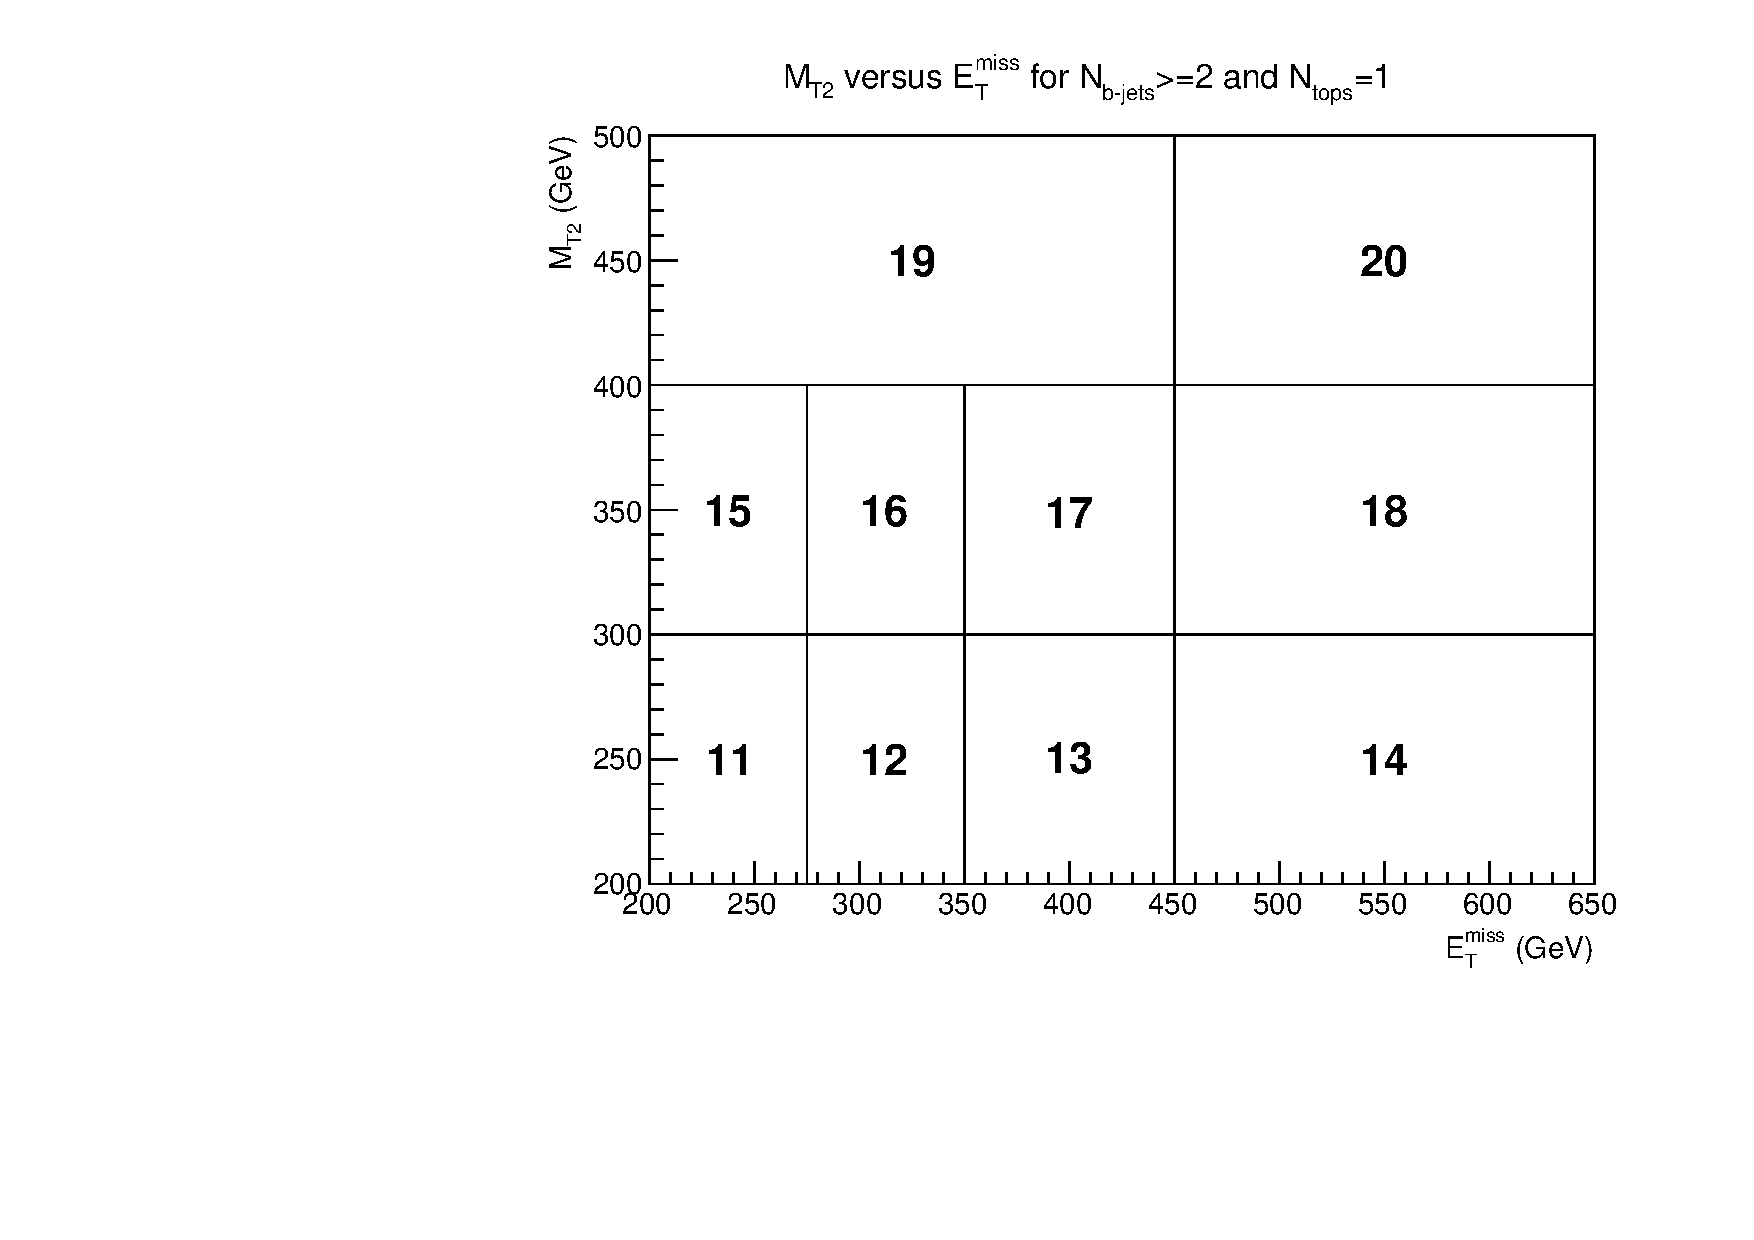
\includegraphics[width=0.45\linewidth]{HadStopPaper/figures/poly_MT2_vs_met_merged_1.pdf} \\
    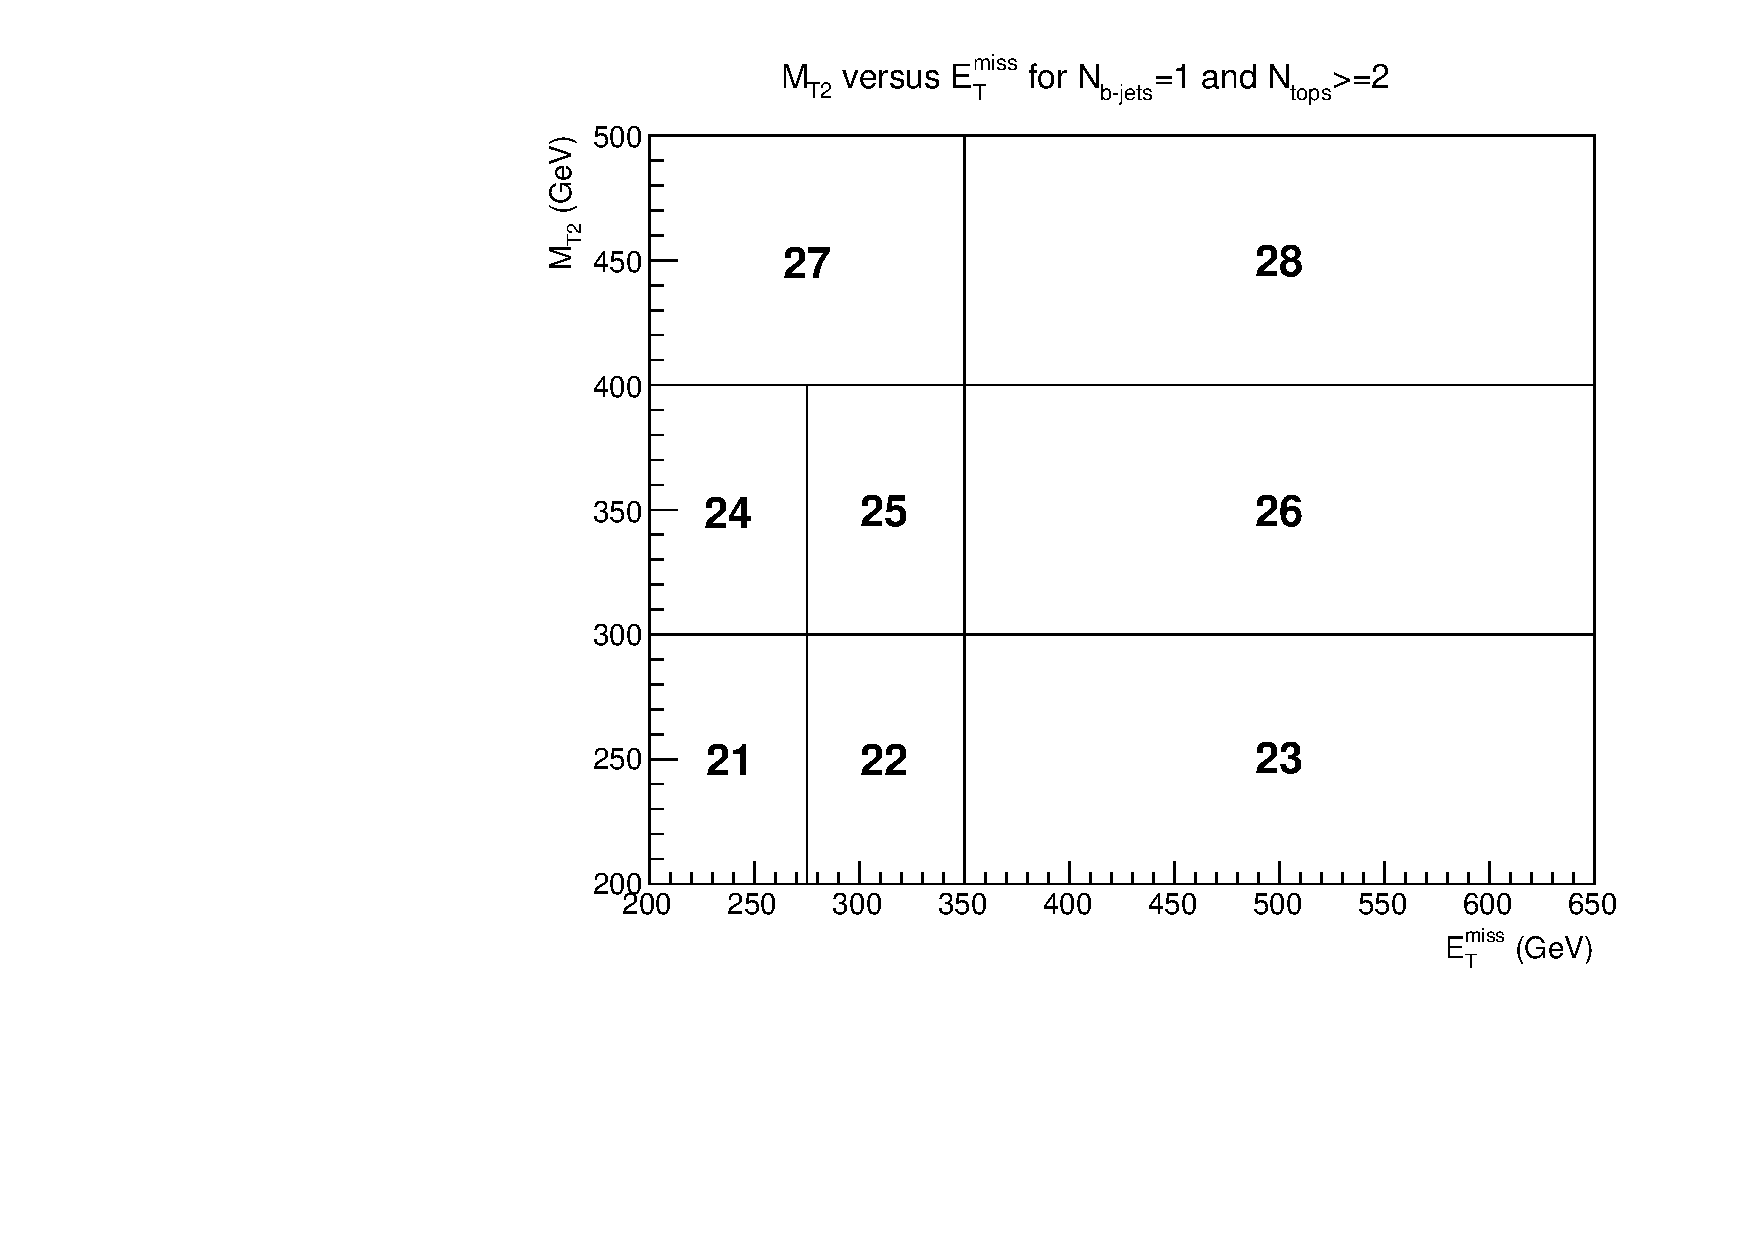
\includegraphics[width=0.45\linewidth]{HadStopPaper/figures/poly_MT2_vs_met_merged_3.pdf} 
    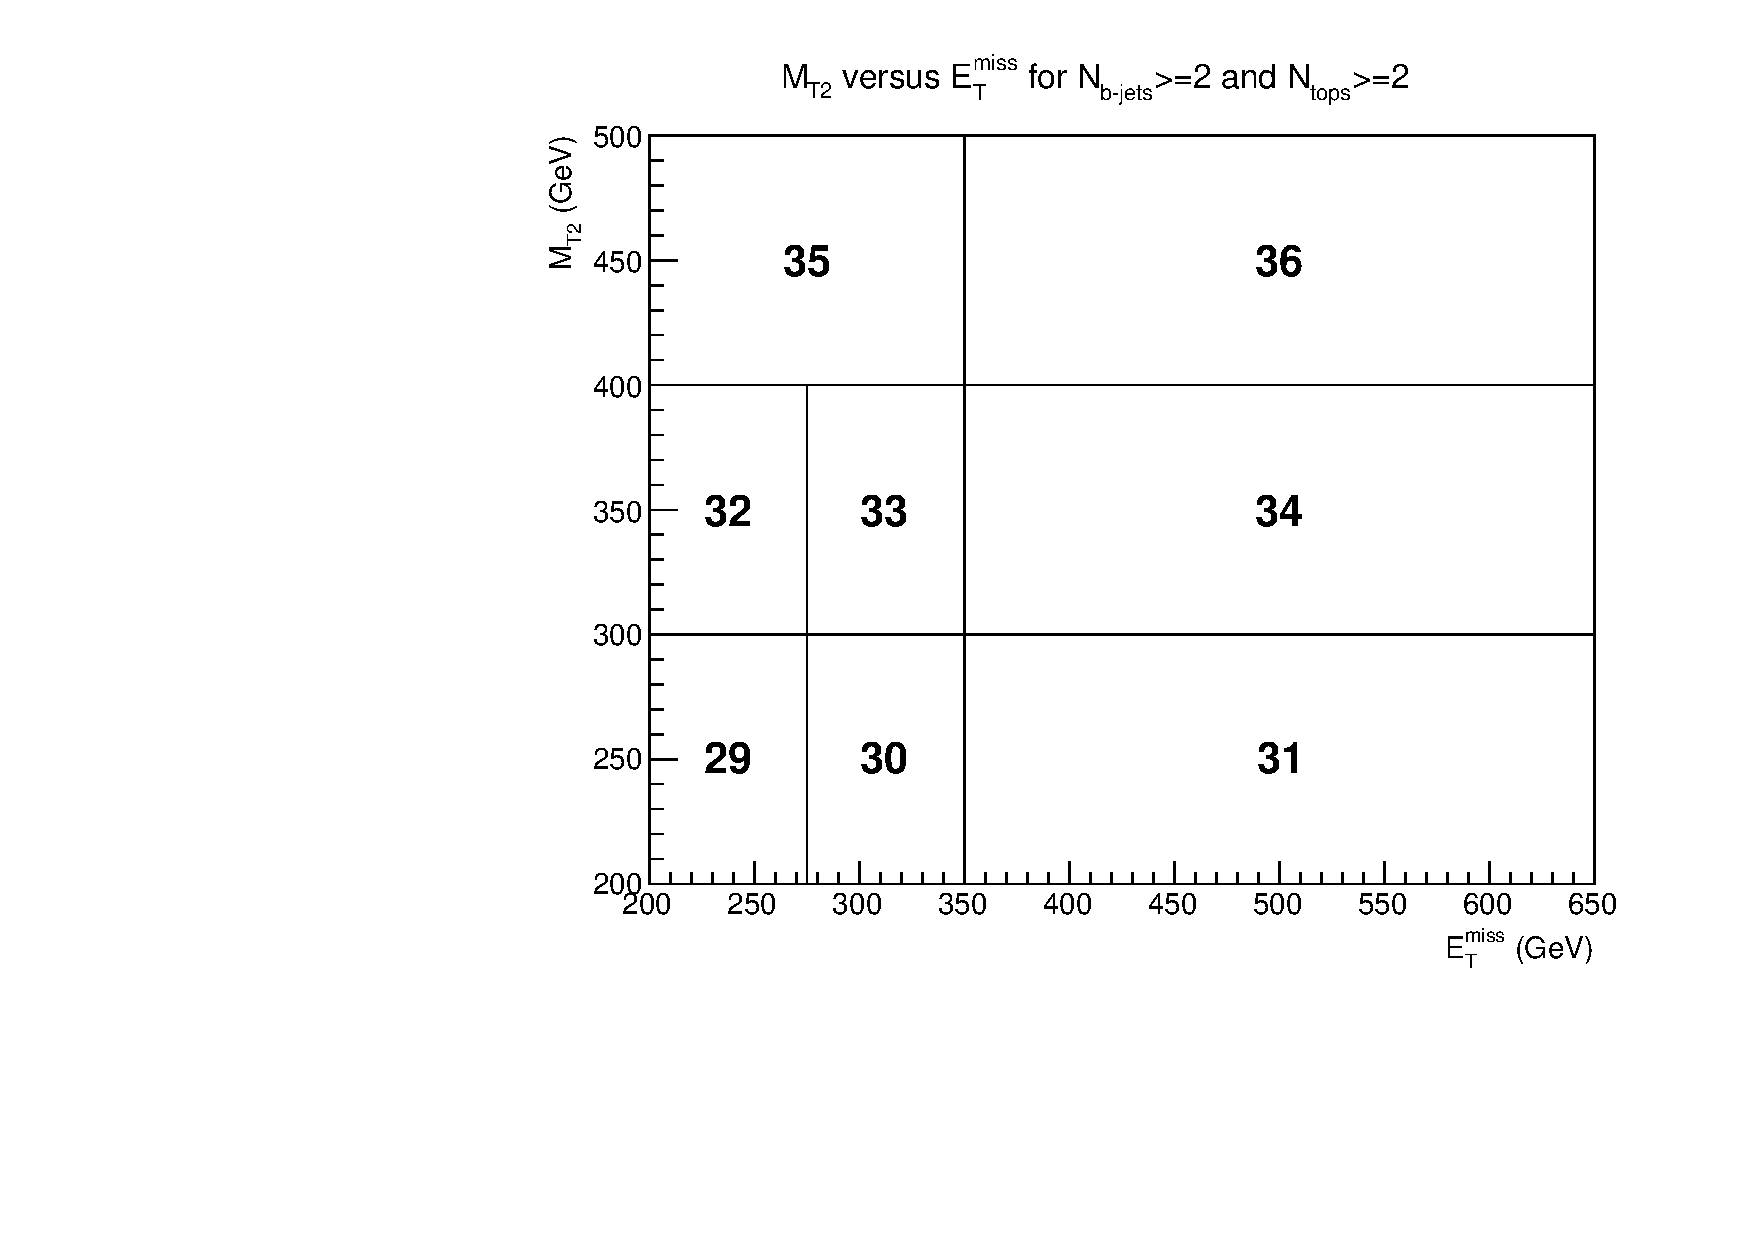
\includegraphics[width=0.45\linewidth]{HadStopPaper/figures/poly_MT2_vs_met_merged_4.pdf} \\
    \caption{ Search bin definitions after baseline selection cuts. }
    \label{fig:hadstopArray}
  \end{center}
\end{figure}

The most significant background comes from the SM t$\bar{\text{t}}$ production or W-boson production in association with jets, where the ${\rm W}$ decays into leptons that are either not accepted, not reconstructed, or not isolated. The next largest contribution comes from $\zinv$ production in association with jets, including b-jets, in which the neutrino pair gives rise to large $\met$ and the top quark conditions are satisfied by an accidental combination of the jets. The QCD multi-jet contribution and the contribution from other rare SM processes are subdominant across all search bins. 


\subsubsection{Background estimation}
The t$\bar{\text{t}}$, W$+$jets, and QCD backgrounds are estimated by data-driven methods detailed in \cite{CMS:2016nhb}, but are not discussed thoroughly here. The $\zinv$ background is most dominant in regions of small $\Ht$ and large $\met$, and the bin-by-bin estimation is detailed here.

The $\zinv$ background is estimated using the ee and $\mu\mu$ samples as a proxy for the true sample in which the Z decays into neutrinos. The method used to derive the prediction, as well as uncertainties, is that described in Section \ref{sec:zinv}. The values and uncertainties in the bin-by-bin prediction are shown in Fig. \ref{fig:2015ZinvPrediction} for the $\mu\mu$-derived prediction, the ee-derived prediction, and the prediction based on the combined $\mu\mu+$ee sample. 
\begin{figure}[tb!]
\centering
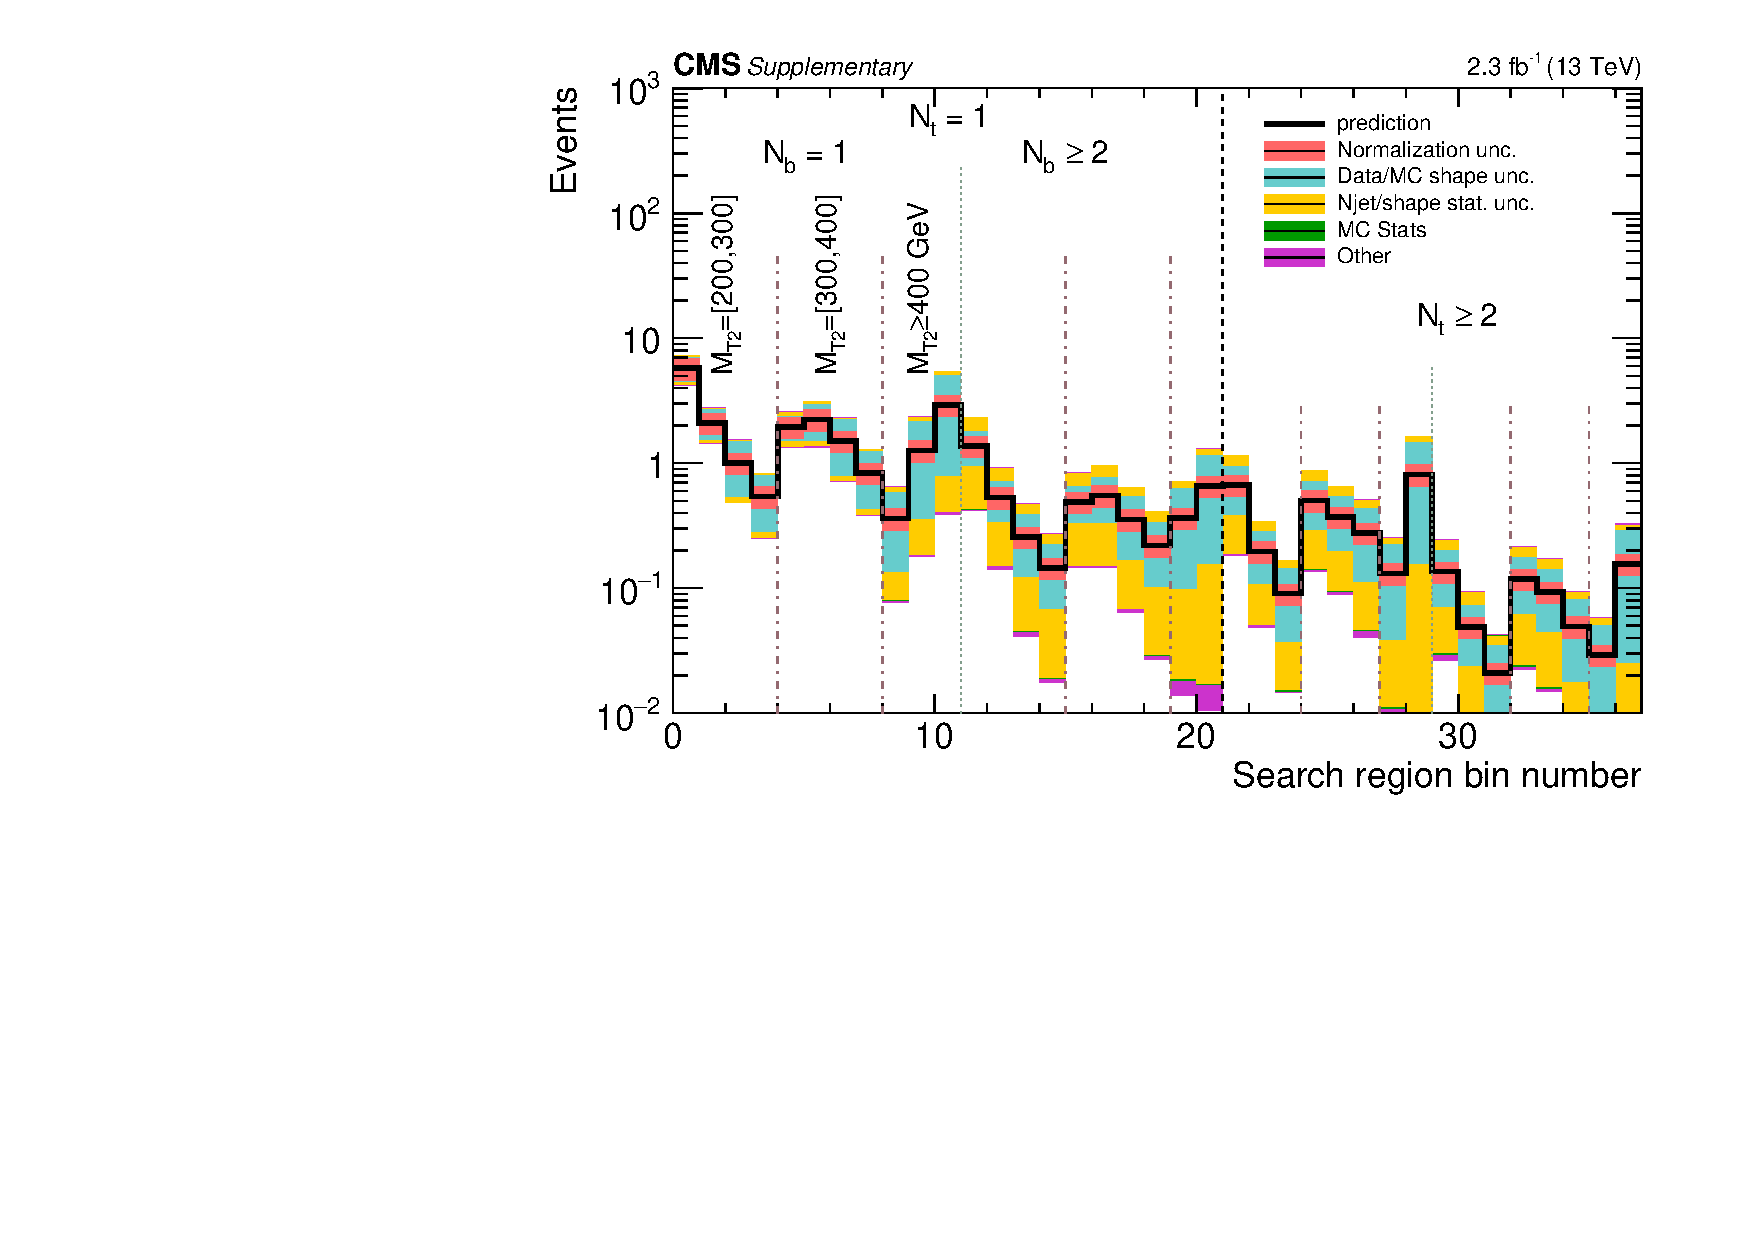
\includegraphics[width=0.6\linewidth]{figures/SusySearches/HadStop2015/moneyplotJoeMu.pdf}\\
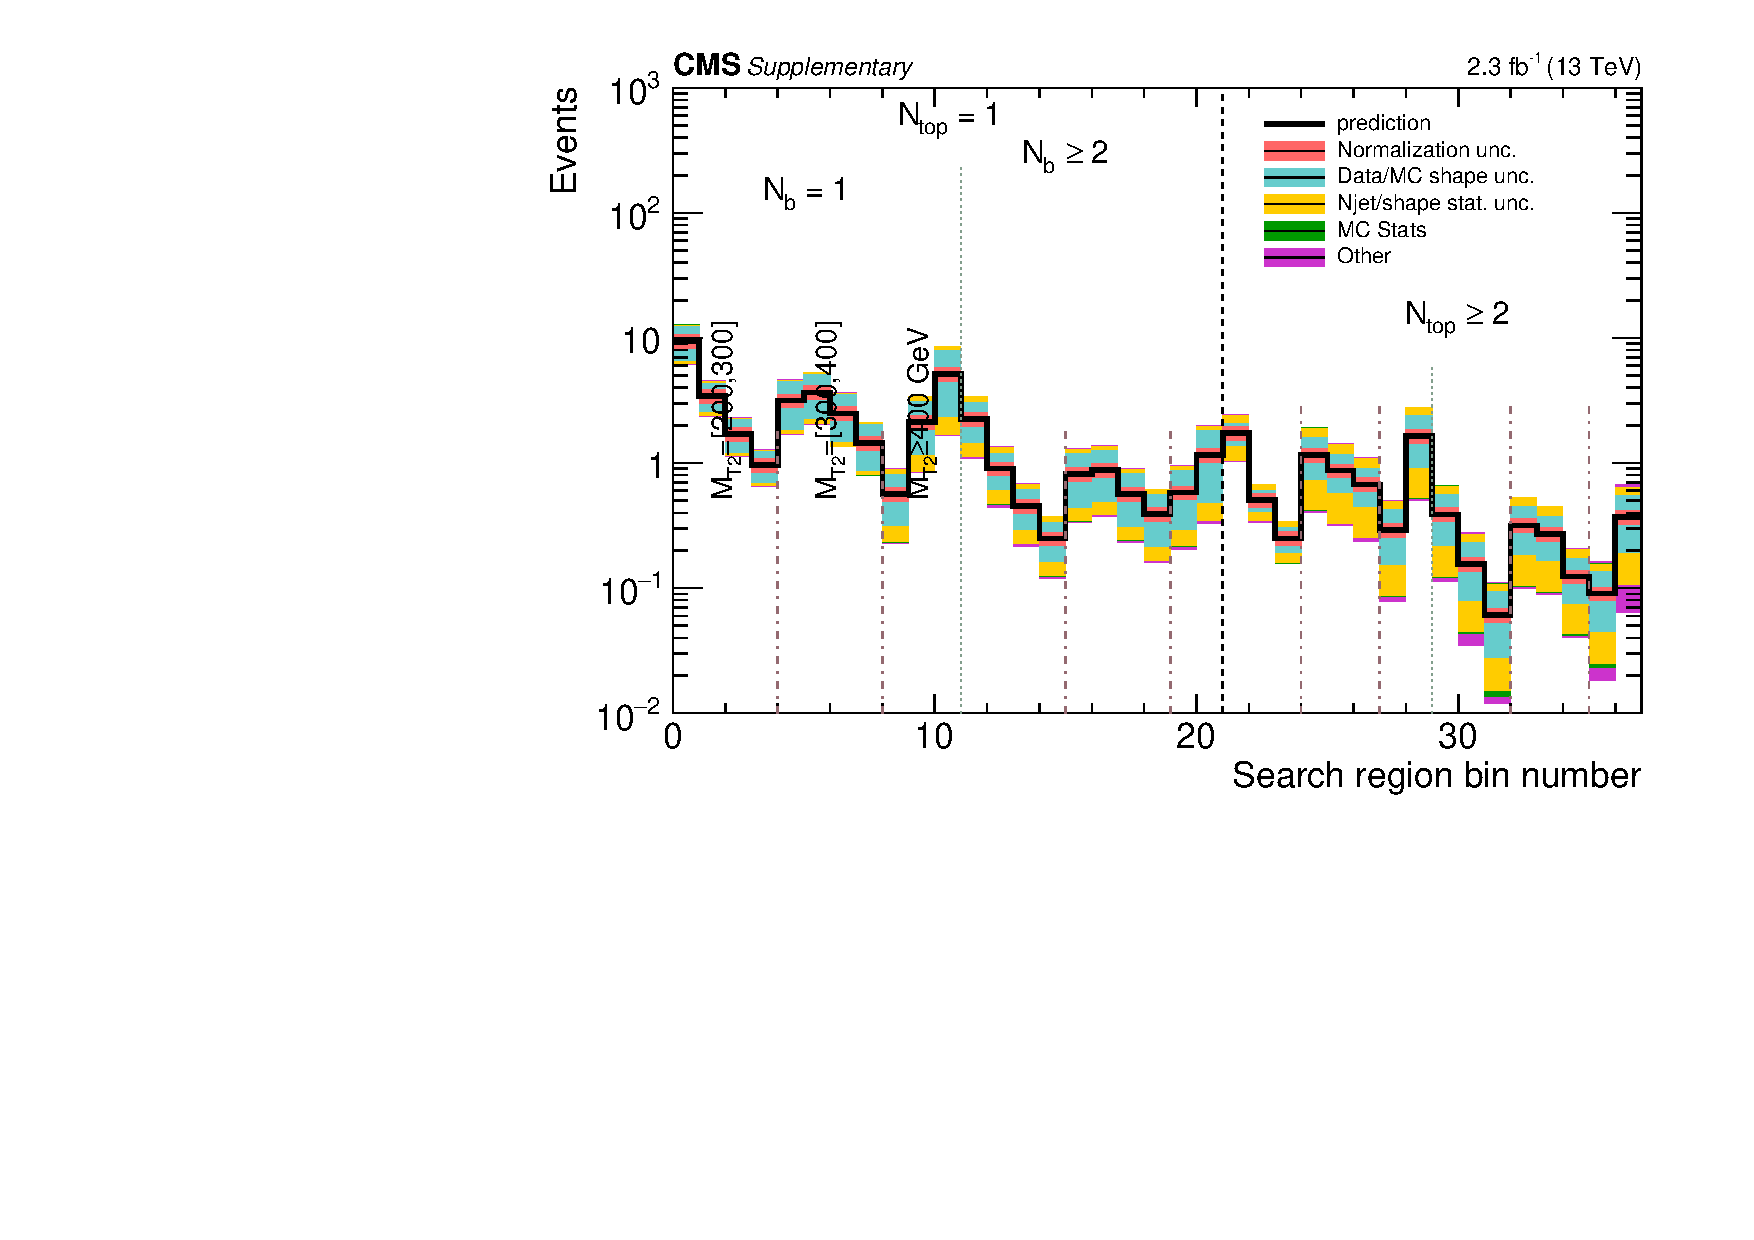
\includegraphics[width=0.6\linewidth]{figures/SusySearches/HadStop2015/moneyplotEl.pdf}\\
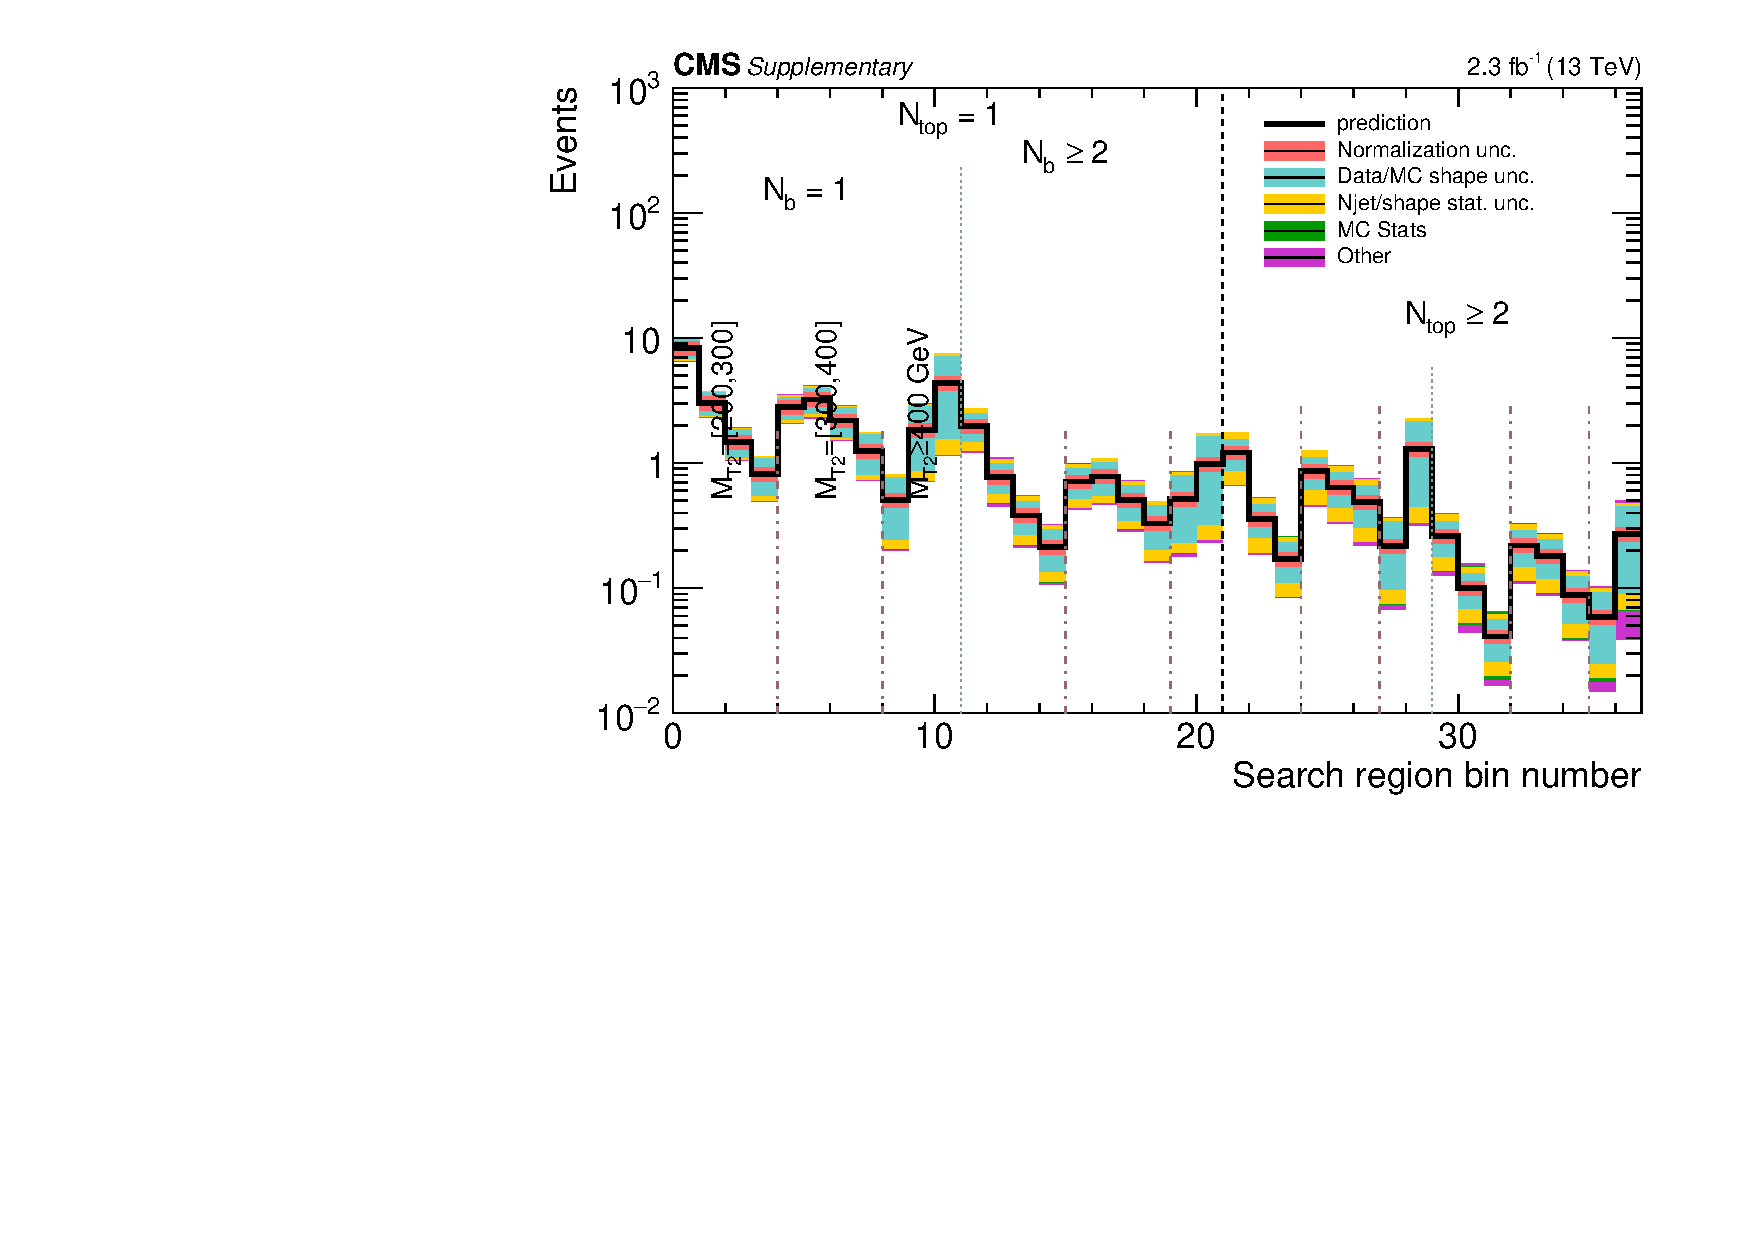
\includegraphics[width=0.6\linewidth]{figures/SusySearches/HadStop2015/moneyplotLep.pdf}
\caption{ The predicted counts originating from standard model $\zinv$ production, based on the $\mu\mu$ sample (top), the ee sample (center), and the combined $\mu\mu+$ee sample (bottom). Each type of uncertainty, described in Section \ref{sec:zinv}, appears as a color-filled rectangle centered on the predicted value, summed in quadrature with the inner uncertainties. }
\label{fig:2015ZinvPrediction}
\end{figure}
The $\mu\mu$-derived and ee-derived predictions are compatible within the uncertainties, but the ee-derived prediction is systematically larger than that of the $\mu\mu$-derived prediction by at least 40\%. This is due to the difference in the normalization factor-derived in the two methods, as well as differences in the data-simulation weights. 


\subsubsection{Results and interpretation}
The predicted number of SM background events and the number of events observed in data for each of the search bins are shown in Figure~\ref{fig:baseline_SR} and Tabulated in Ref.~\cite{CMS:2016nhb}. 
\begin{figure}[htbp]
  \begin{center}
  \begin{tabular}{cc}
\hspace{-1.5cm}
  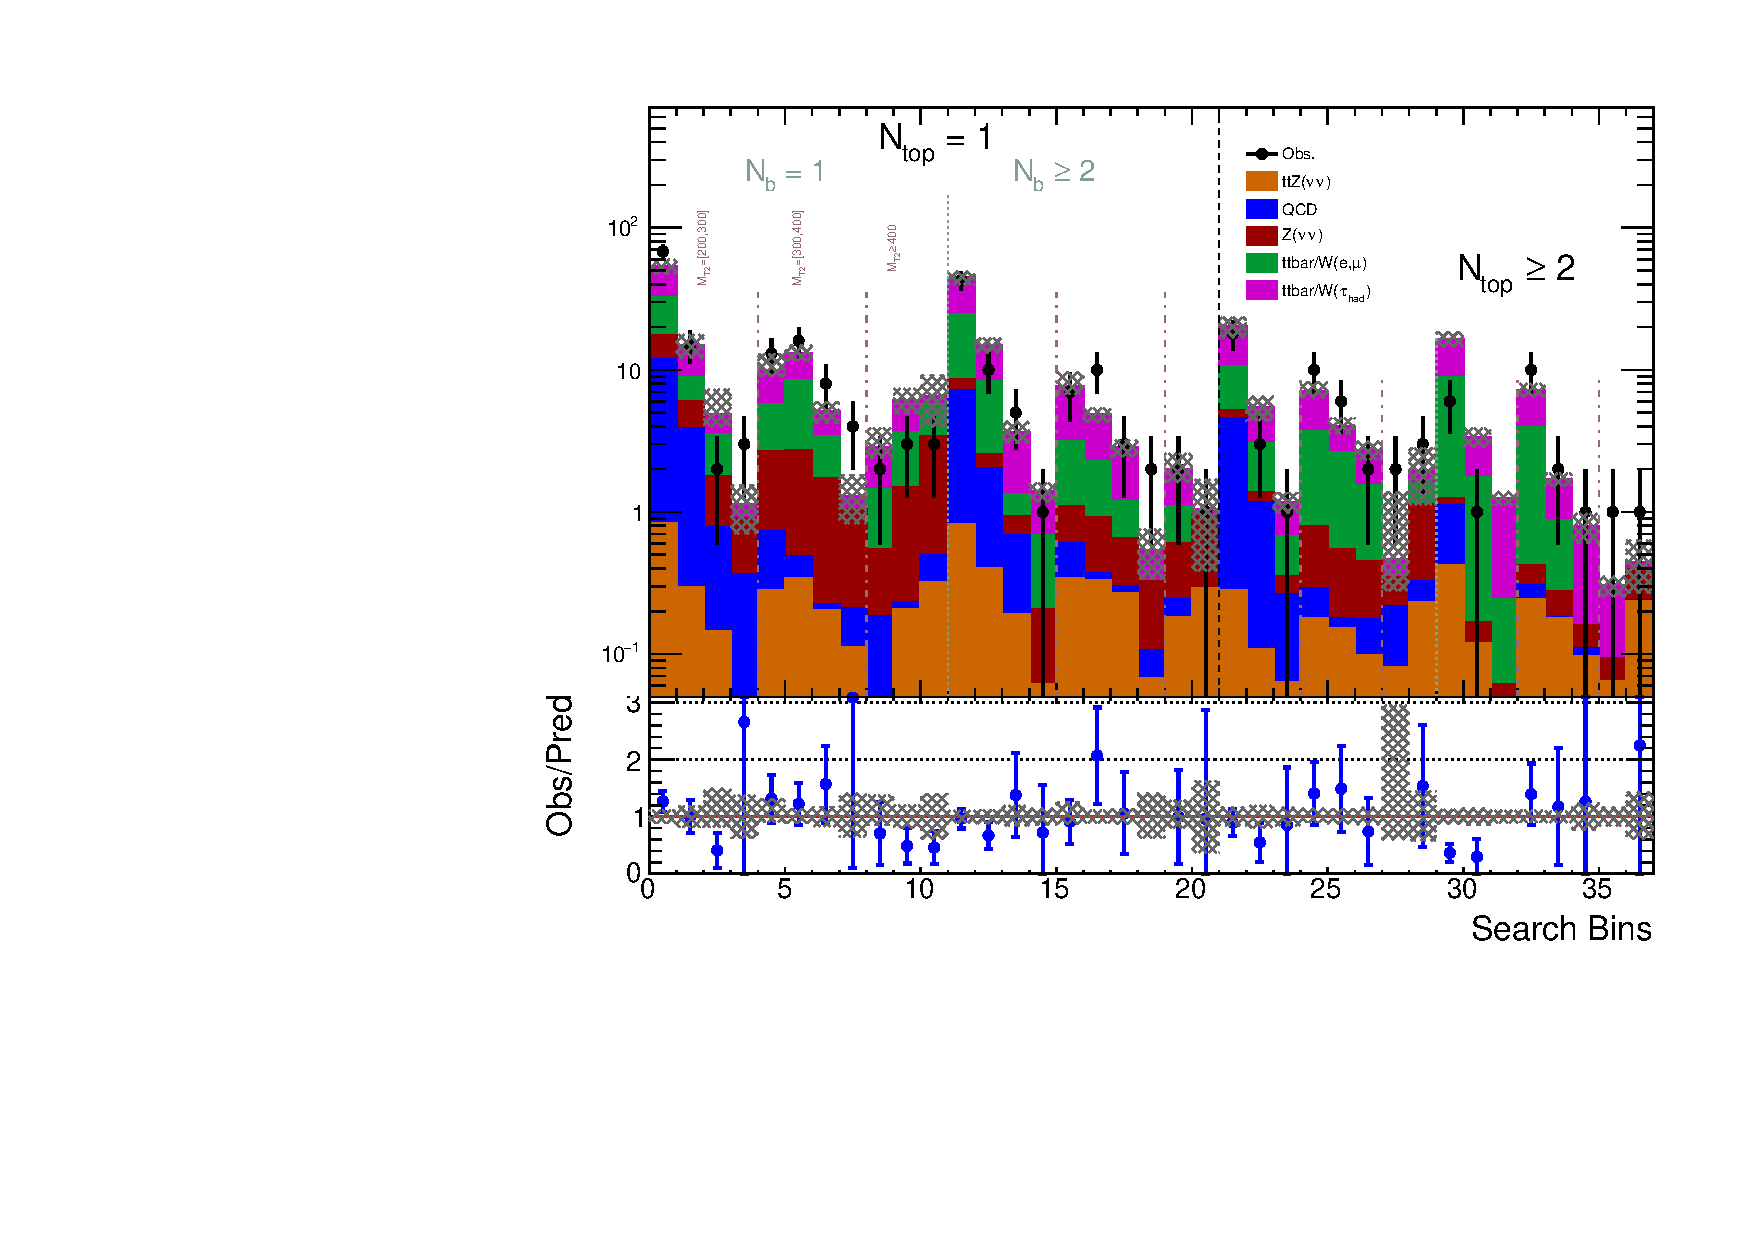
\includegraphics[width=0.85\textwidth]{figures/SusySearches/HadStop2015/UnblindPlots.pdf}
  \end{tabular}
  \caption{Data are shown as black points. The total predictions are shown in filled solid area. The bottom plot shows the ratio of data over total background prediction in each search bin. Only statistical uncertainties are propagated to the ratio. The numbering scheme is given in Ref. \cite{CMS:2016nhb}.}
    \label{fig:baseline_SR}
  \end{center}
\end{figure}
The predicted background counts are observed to be compatible with the data in all 37 regions, within uncertainties. Therefore, no evidence of new physics is observed.
These results are interpreted in the context of the simplified models shown in Fig. \ref{fig:Ra2bSMS}.

%The following uncertainties on the signal modeling are taken into account when the limits are determined: simulation sample size, luminosity determination ($4.6\%$), lepton and isolated track veto, b-tag efficiency corrections used to scale simulation to data, trigger efficiency, QCD renormalisation and factorization scales, initial/final state radiation (ISR/FSR), signal acceptance and efficiency arising from the jet energy-momentum corrections, jet energy-momentum resolutions, and propagated to \MET, parton distribution functions (PDF) of the proton

The results are interpreted in terms of the simplified model scenarios shown in Fig. \ref{fig:hadstopSMS} using an analogous limit setting procedure discussed in Section \ref{sec:ra2b2015}. Uncertainties in the signal yields are similar to those discussed in Section \ref{sec:ra2b2015}, with additional uncertainties associated with differences in the top-quark tagging efficiency and false positive rate between the CMS fast and full simulations, on the order of a few percent.

%%%%%%%%%%%%%%%%%%%%%%%%%%%%%%%%%%%%%%%%%%%%%%%%%%

%-------------
Upper limits on the observed cross section for the signal models T2tt and T1tttt are shown in Figs. \ref{fig:fulllimit_T2tt} and \ref{fig:fulllimit_T1tttt}, along with contours corresponding to the expected (red) and expected (black) upper limits on the SUSY masses, assuming the assuming the NLO+NLL theoretical SUSY cross sections. In the case of T2tt, limits are shown assuming the predicted $\zinv$ counts based on the $\mu\mu$, ee, and $\mu\mu+$ee samples. For T1tttt, just the limits on the $\mu\mu$ and $\mu\mu+$ee samples are shown. 

%%%%%%%%%%%%%%%%%%%%%%%%%%%%%%%%%%%%%%%%%%%%%%%%%%
\begin{figure}[htbp]
  \begin{center}
  \begin{tabular}{cc}
\hspace{-1.5cm}
  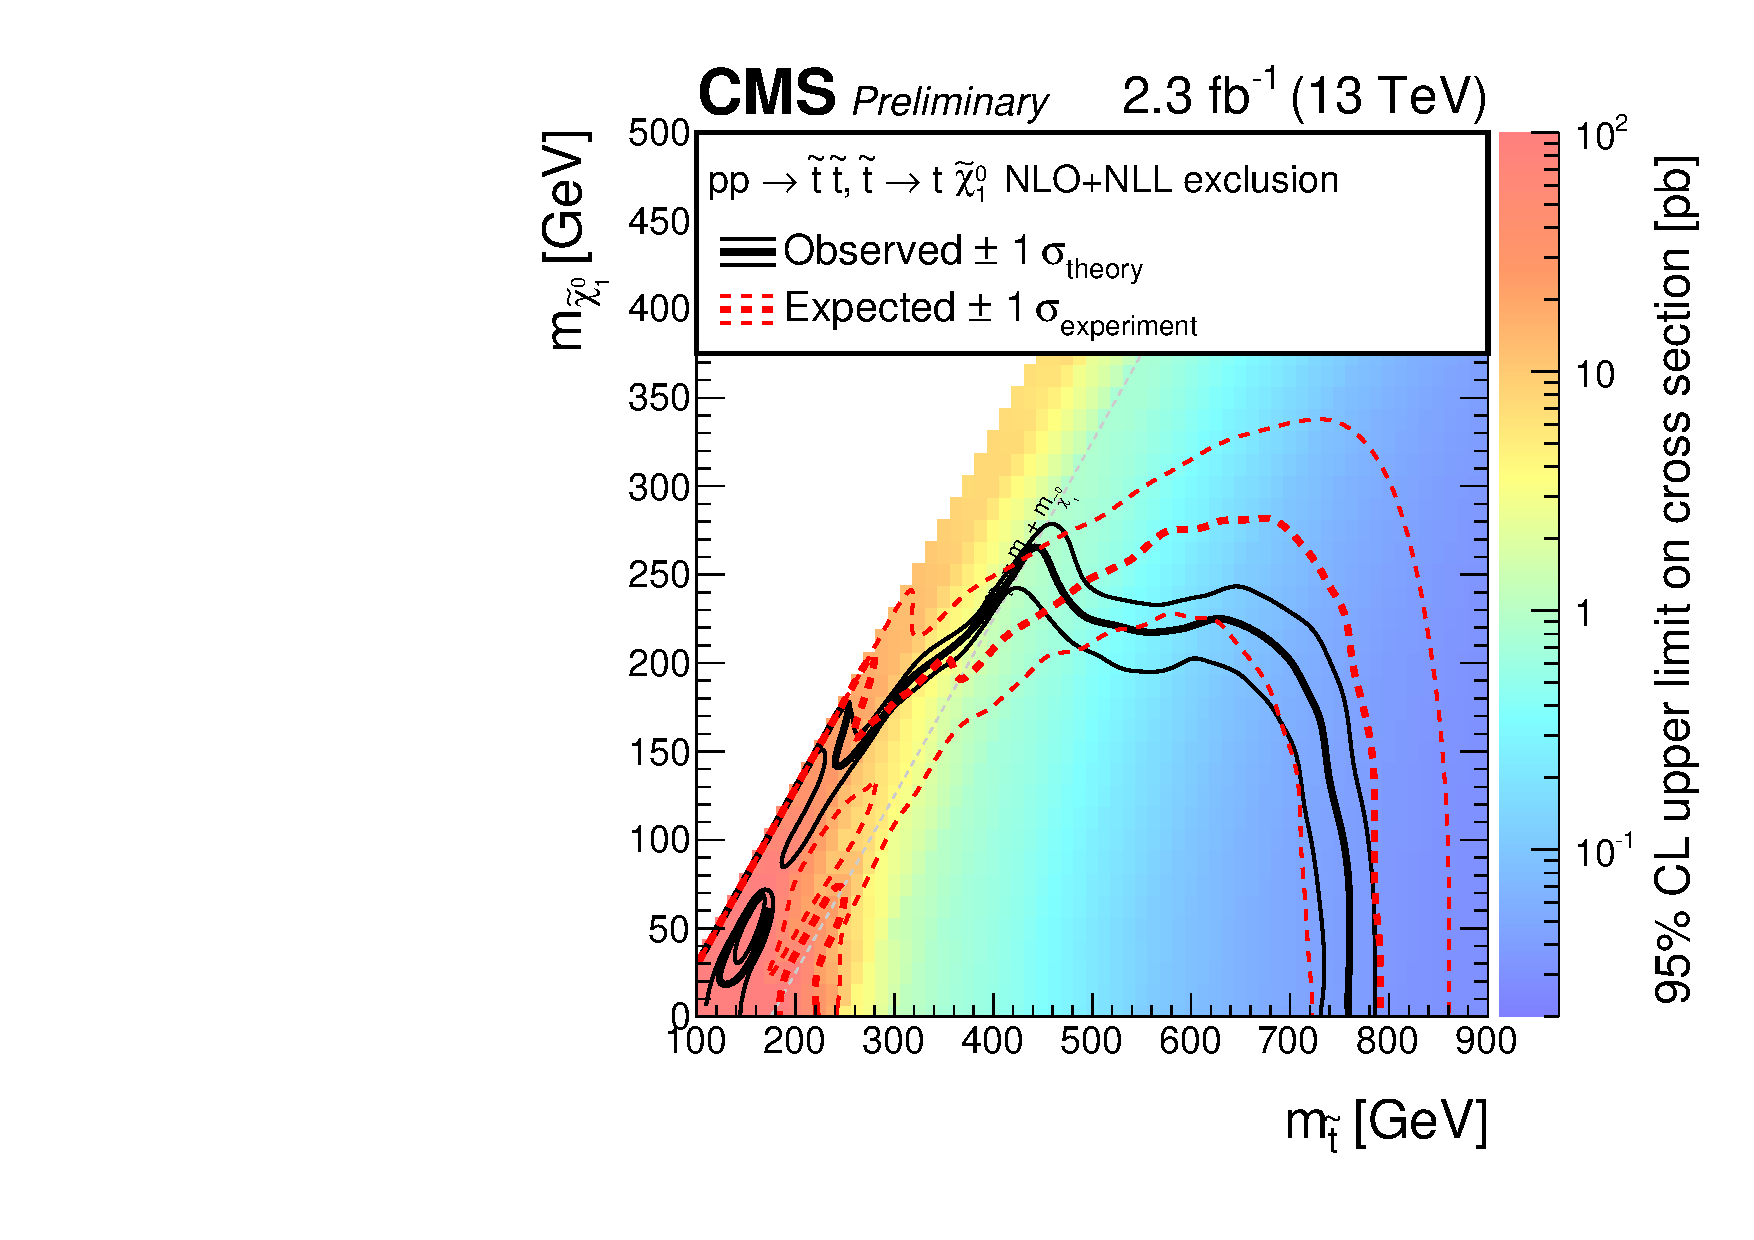
\includegraphics[angle=0,width=0.48\textwidth]{figures/SusySearches/HadStop2015/HadStopT2tt_Mu.pdf}
  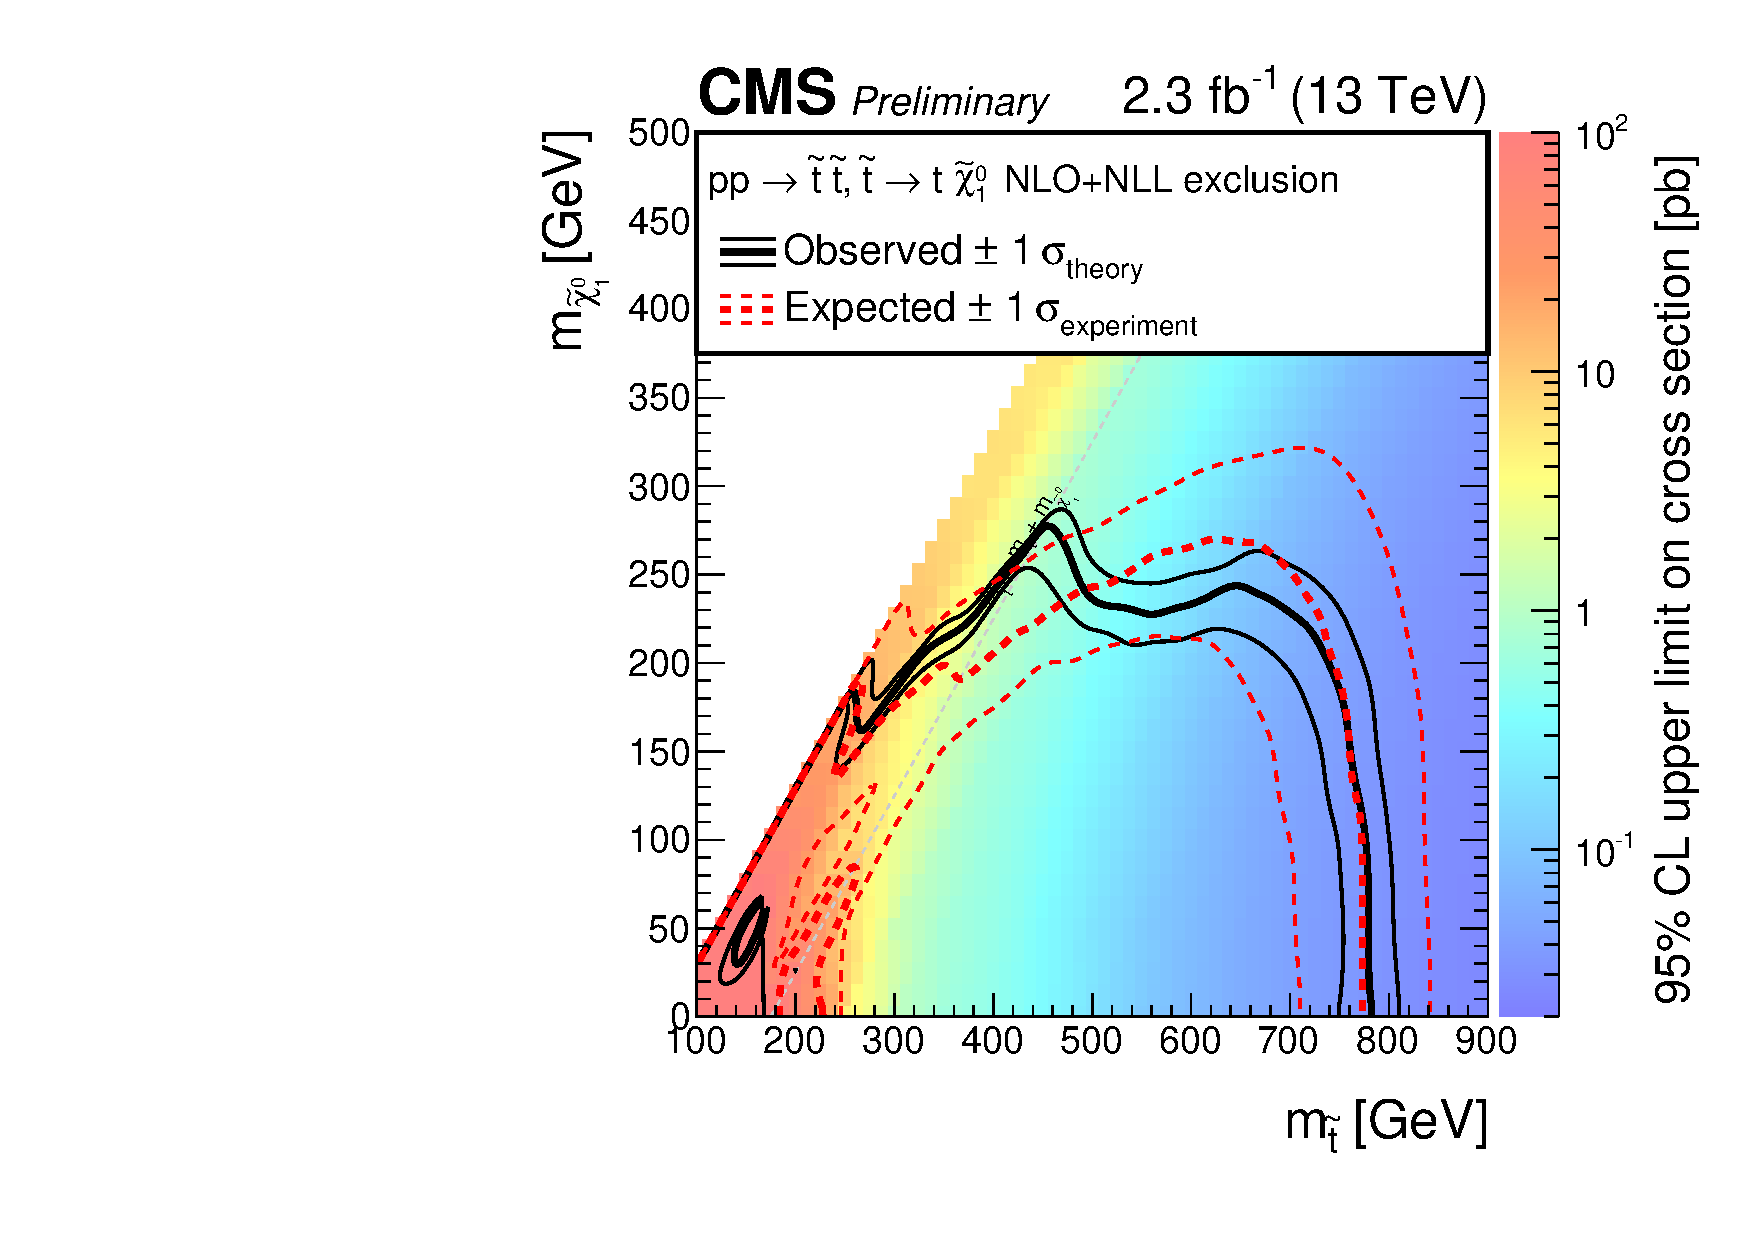
\includegraphics[angle=0,width=0.48\textwidth]{figures/SusySearches/HadStop2015/HadStopT2tt_El.pdf}\\
    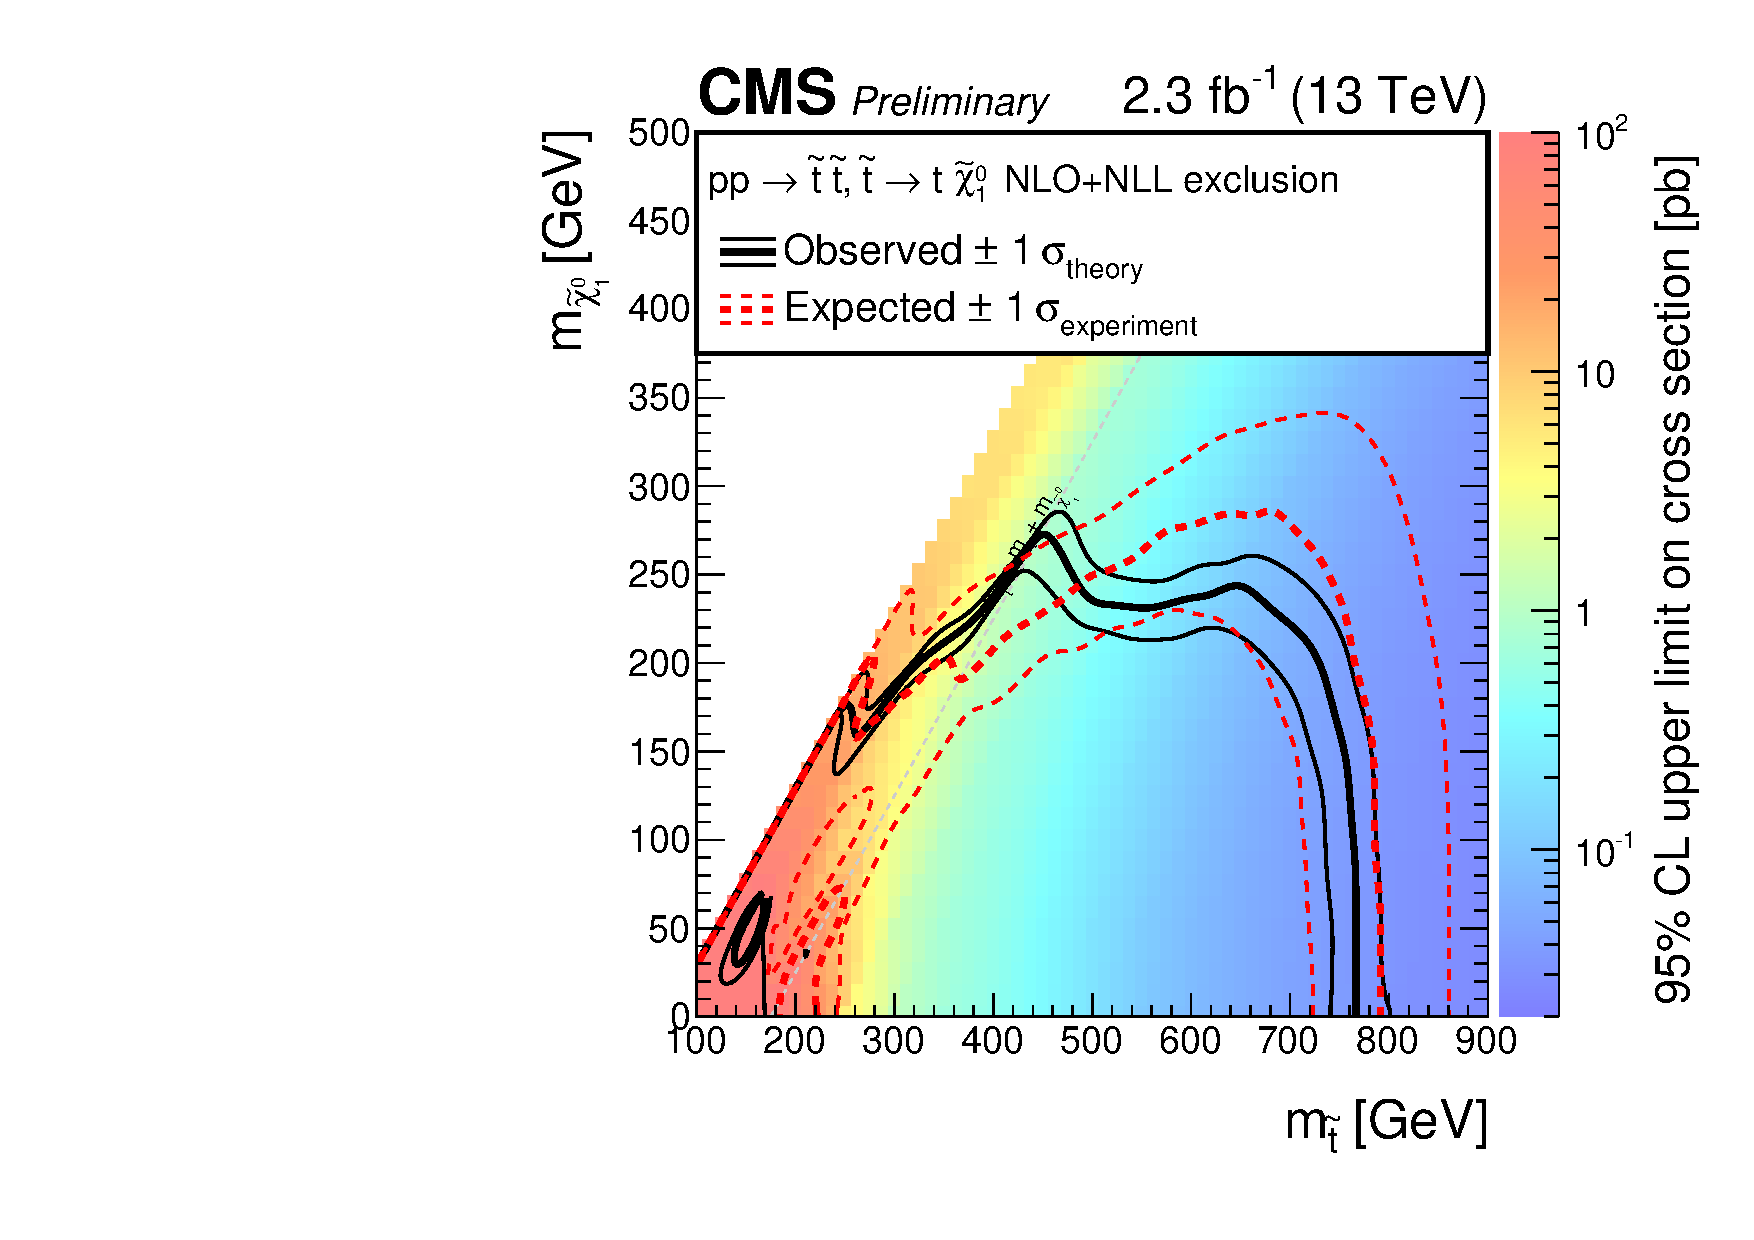
\includegraphics[angle=0,width=0.48\textwidth]{figures/SusySearches/HadStop2015/HadStopT2tt_MuEl.pdf}
  \end{tabular}
  \caption{Observed (black contour) and expected (red contour) limits on the top squark and LSP masses in the context of the T2tt model. The top-left plot corresponds to the $\mu\mu$-derived $\zinv$ prediction, the top-right to the ee-derived prediction, and the bottom plot to the prediction of the combined $\mu\mu+$ee sample.}
    \label{fig:fulllimit_T2tt}
  \end{center}
\end{figure}

\begin{figure}[htbp]
  \begin{center}
  \begin{tabular}{cc}
\hspace{-1.5cm}
  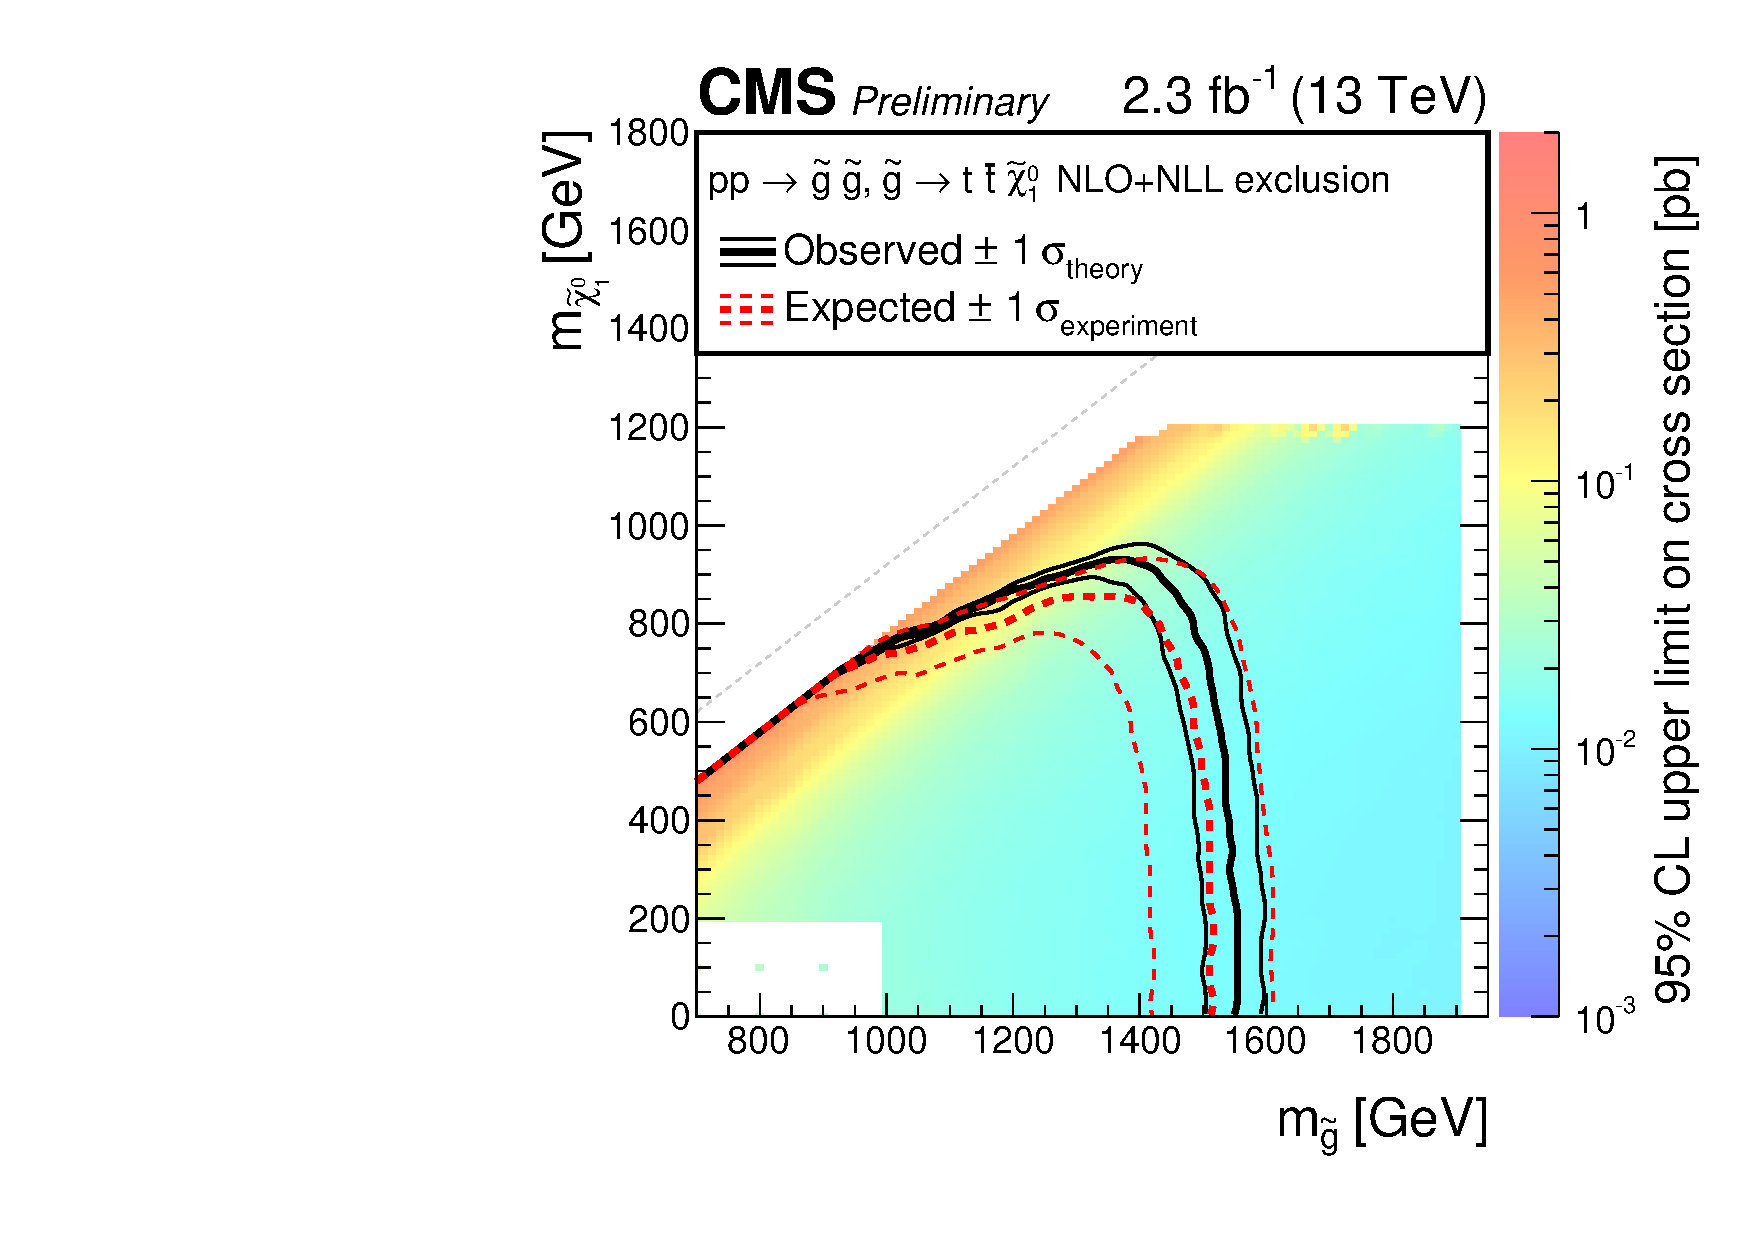
\includegraphics[angle=0,width=0.48\textwidth]{figures/SusySearches/HadStop2015/HadStopT1tttt_Mu.pdf}
  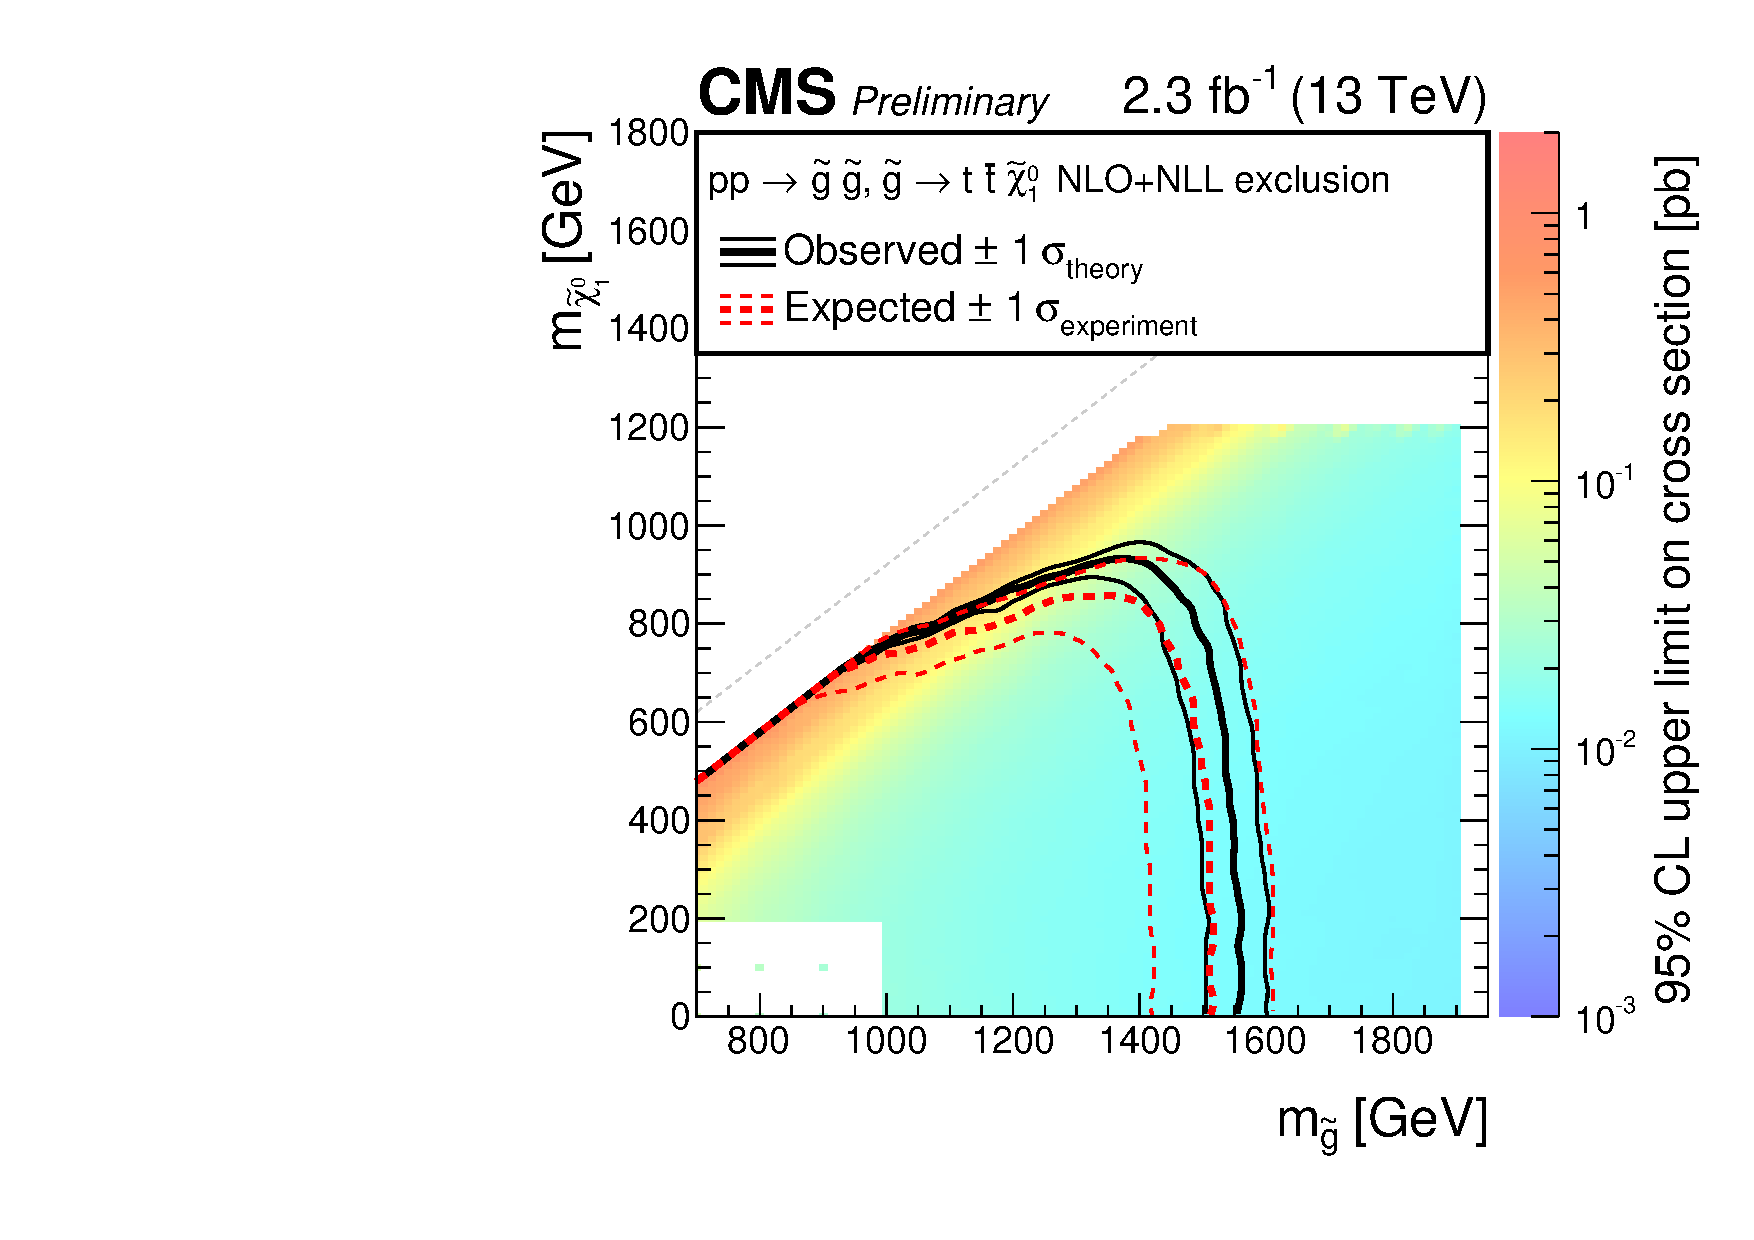
\includegraphics[angle=0,width=0.48\textwidth]{figures/SusySearches/HadStop2015/HadStopT1tttt_MuEl.pdf}
  \end{tabular}
  \caption{Observed (black contour) and expected (red contour) limits on the gluino and LSP masses in the context of the T1tttt model. The left plot corresponds to the $\mu\mu$-derived prediction for the $\zinv$ counts, and the right plot to the muon$+$ee-derived prediction.}
    \label{fig:fulllimit_T1tttt}
  \end{center}
\end{figure}
%%%%%%%%%%%%%%%%%%%%%%%%%%%%%%%%%%%%%%%%%%%%%%%%%%
In the case of T2tt, the ee-derived expected limit is somewhat less constraining than that of the expected muon-derived limit, as was expected from the outset. The ee-derived observed limit on the top squark mass is actually stronger than the $\mu\mu$-derived observed limit by about 20 GeV, for small values of the LSP mass. This difference is owing to the considerably larger ee-derived $\zinv$ prediction. The combined $\mu\mu$+ee-derived expected limit is comparable to the $\mu\mu$-derived expected limit. The observed limit based on the combined result is slightly more constraining on the top squark mass than the $\mu\mu$ result, by about 10 GeV, for small LSP masses. The largest observed upper limit on $m_{\tilde{\text{t}}}$ for low LSP mass comes from the ee estimate, and is approximately 780 GeV, coinciding with the expected limit. In the compressed region, the strongest observed limit comes from the ee prediction, where LSPs are excluded with masses below about 180 GeV, which is nearly in agreement with the expected limit.

In the T1tttt model, only negligible differences appear between the $\mu\mu$ and the combined $\mu\mu+$ee predictions. Given the limited constraining power of the ee control sample, this sample be be better used in more creative ways, for example, as a training sample for a multivariate discriminant. This is explored in the next chapter.

